\let\negmedspace\undefined
\let\negthickspace\undefined
\documentclass[journal]{IEEEtran}
\usepackage[a5paper, margin=10mm, onecolumn]{geometry}
%\usepackage{lmodern} % Ensure lmodern is loaded for pdflatex
\usepackage{tfrupee} % Include tfrupee package

\setlength{\headheight}{1cm} % Set the height of the header box
\setlength{\headsep}{0mm}     % Set the distance between the header box and the top of the text

\usepackage{gvv-book}
\usepackage{gvv}
\usepackage{cite}
\usepackage{amsmath,amssymb,amsfonts,amsthm}
\usepackage{algorithmic}
\usepackage{graphicx}
\usepackage{textcomp}
\usepackage{xcolor}
\usepackage{txfonts}
\usepackage{listings}
\usepackage{enumitem}
\usepackage{mathtools}
\usepackage{gensymb}
\usepackage{tfrupee}
\usepackage[breaklinks=true]{hyperref}
\usepackage{tkz-euclide} 
\usepackage{listings}
% \usepackage{gvv}                                        
\def\inputGnumericTable{}                                 
\usepackage[latin1]{inputenc}                                
\usepackage{color}                                            
\usepackage{array}                                            
\usepackage{longtable}                                       
\usepackage{calc}                                             
\usepackage{multirow}                                         
\usepackage{hhline}                                           
\usepackage{ifthen}                                           
\usepackage{lscape}
\usepackage{circuitikz}
\usepackage{comment}
\tikzstyle{block} = [rectangle, draw, fill=blue!20, 
    text width=4em, text centered, rounded corners, minimum height=3em]
\tikzstyle{sum} = [draw, fill=blue!10, circle, minimum size=1cm, node distance=1.5cm]
\tikzstyle{input} = [coordinate]
\tikzstyle{output} = [coordinate]


\begin{document}

\bibliographystyle{IEEEtran}
\vspace{3cm}

\title{5.8.16}
\author{EE25BTECH11018-Darisy Sreetej}
 \maketitle
% \newpage
% \bigskip
{\let\newpage\relax\maketitle}

\renewcommand{\thefigure}{\theenumi}
\renewcommand{\thetable}{\theenumi}
\setlength{\intextsep}{10pt} % Space between text and floats


\numberwithin{equation}{enumi}
\numberwithin{figure}{enumi}
\renewcommand{\thetable}{\theenumi}

\textbf{Question}:
The taxi charges in a city consist of a fixed charge together with the charges for the distance covered. For a distance of 10 km, the charge paid is \rupee105 and for a distance of 15 km, the charge paid is \rupee155. What are the fixed charges and the charge per km? How much does a person have to pay for travelling a distance of 25 km ?\\
\textbf{Solution}:\\
Let us solve the given question theoretically and then verify the solution computationally.\\
Let
x = fixed charge , 
y = charge per km \\
Then total fare = $x + y \times distance$\\
According to the question,
The equation of lines given
\begin{align}
    \myvec{1&&10}\vec{x}=105 \\
    \myvec{1&&15}\vec{x}=115 
    \end{align}
    where ,\quad $\vec{x}=\myvec{x\\y}$\\
From the question ,
\begin{align}
     \myvec{1&&25}\vec{x}=c 
     \end{align}
      where ,\quad $c$ = total fare the person should pay for travelling 25 km
\begin{align}
    \therefore \myvec{1&&10\\1&&15\\1&&25}\vec{x}=\myvec{105\\155\\c}
\end{align}
Using augmented matrix,
\begin{align}
    \augvec{2}{1}{1&10&105\\1&15&155\\1&25&c}
\end{align}
Upon doing row reduction,
\begin{align}
\begin{aligned}
       \augvec{2}{1}{1&10&105\\1&15&155\\1&25&c}
     \xleftrightarrow{R_3 = R_3 - R_1}
       \augvec{2}{1}{1&10&105\\1&15&155\\0&15&c-105}
\end{aligned}
\end{align}
\begin{align}
\begin{aligned}
      \augvec{2}{1}{1&10&105\\1&15&155\\0&15&c-105}
     \xleftrightarrow{R_2 = R_2 - R_1}
       \augvec{2}{1}{1&10&105\\0&5&50\\0&15&c-105}
\end{aligned}
\end{align}
\begin{align}
\begin{aligned}
      \augvec{2}{1}{1&10&105\\0&5&50\\0&15&c-105}
     \xleftrightarrow{R_3 = R_3 - 3 \times R_2}
     \augvec{2}{1}{1&10&105\\0&5&50\\0&0&c-255}
\end{aligned}
\end{align}
From (0.8),
\begin{align}
    \begin{aligned}
        0=c-255\\
        c=255\\
    \end{aligned}
\end{align}
\begin{align}
    \begin{aligned}
       5y=50\\
       y=10\\
       x+10y=105\\
       x=5
    \end{aligned}
\end{align}
\begin{align}
    \implies \vec{x}=\myvec{5\\10}
\end{align}
Thus , fixed charge =\rupee5\\
charge per km = \rupee10\\
The total fare the person should pay for travelling 25 km = \rupee255
\newpage
From the figure, it is clearly verified that the theoretical solution matches with the computational solution.

 \begin{figure}[H]
     \centering
     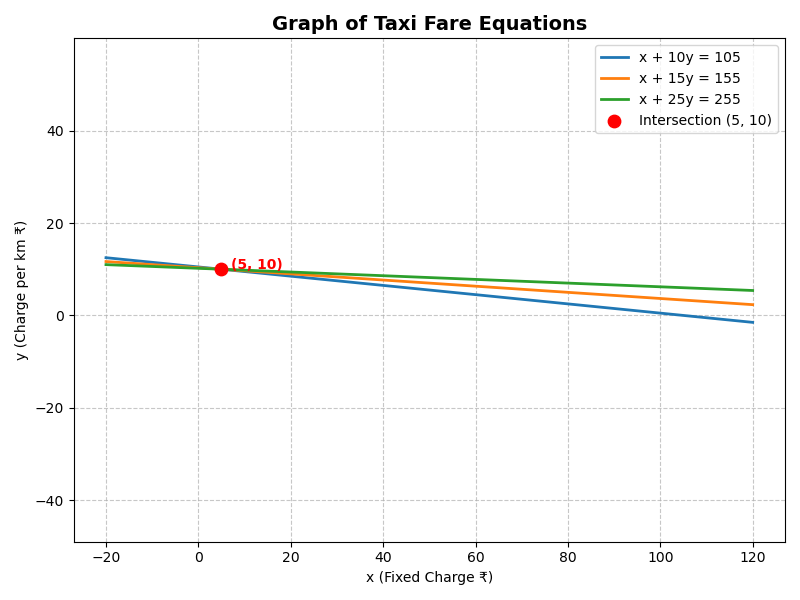
\includegraphics[width=0.8\columnwidth]{figs/fig.png}
     \label{fig:1}
 \end{figure}


\end{document}
